
\subsection{Scheduling}
\label{sec:eval:pal:sched}

This section evaluates several \hostapis{} for scheduling multiple threads
in a \picoproc{},
to create a new thread,
poll an I/O stream (a TCP socket for instance),
and use a synchronization primitive,
such as a notification event or a mutex. 


\begin{figure*}[t!]
\centering
\footnotesize
\resizebox{\textwidth}{!}{%
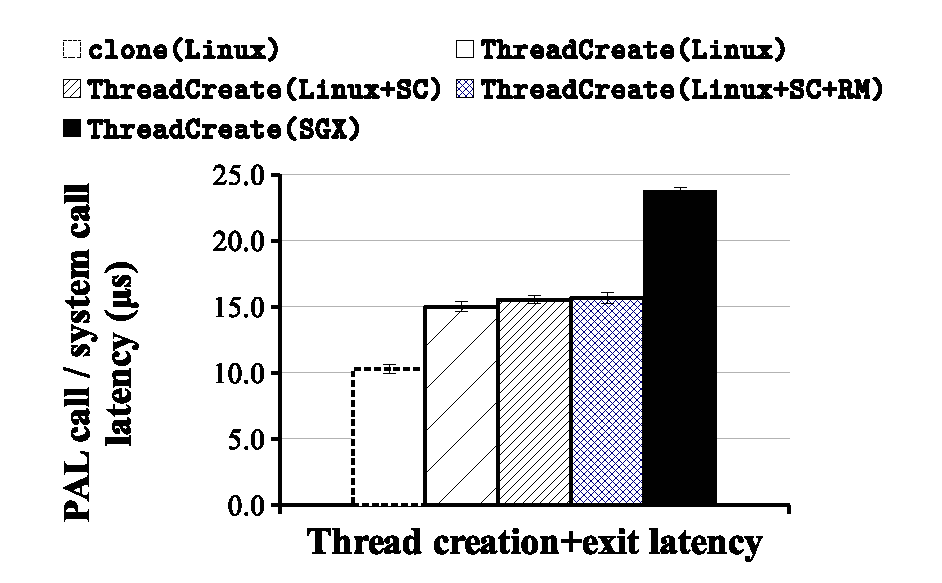
\includegraphics[height=10em]{thread-latency}
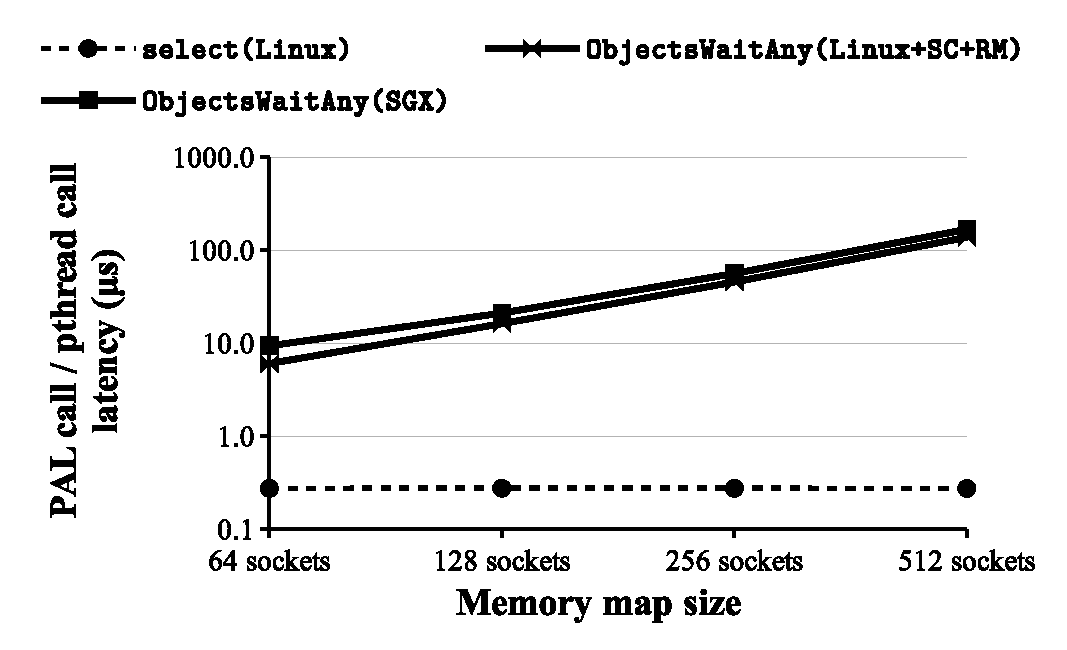
\includegraphics[height=10em]{tcp-select-latency}
}
\parbox{0.49\textwidth}{\centering\bf (a) thread creation}
\parbox{0.49\textwidth}{\centering\bf (b) polling N TCP sockets}
\caption{(a) Thread creation latency and (b) latency of polling a number of TCP sockets.
Lower is better.
The comparison is between (1) \syscall{clone} and \syscall{select} on Linux; (2) \palcall{ThreadCreate} and \palcall{ObjectsWaitAny} on the Linux PAL, with and without a \seccomp{} filter ({\bf +SC}) and reference monitor ({\bf +RM}); (3) the same \hostapis{} on the SGX PAL.}
\label{fig:eval:pal:thread-select-latency}
\end{figure*}


\paragraph{Thread creation.}
%The evaluation shows the latency of creating a new thread within the current process or \picoproc{}.
Figure~\ref{fig:eval:pal:thread-select-latency} (a)
shows the latency of thread creation and exit
on the Linux and SGX PALs,
in comparison with 
\syscall{clone} (with \code{CLONE\_VM})
and \syscall{exit} in a native Linux process.
The latency on the Linux PAL is
%the latency of \palcall{ThreadCreate} and \palcall{ThreadExit} is
\roughly{}46\% higher
than Linux,
%than thread creation and exit on Linux,
and the overhead mainly contributes
to allocating an initial stack for the new thread. %(\palcall{ThreadCreate} does not take an extra argument for specifying the stack address).
The seccomp{} filter and reference monitor
have small impact (less than 5\%)
on the latency of thread creation and exit.


The latency of thread creation on the SGX PAL further includes
the cost of attaching a preallocated enclave thread.
Inside an enclave,
the number of concurrent threads is bound by the number
of TCSes (thread control structure).
To create a new thread,
the SGX PAL has to walk the list of TCSes
to find an unused enclave thread.
%For the SGX PAL, the cost of thread creation is much higher.
%Creating an enclave thread on the SGX PAL takes three primary steps: (1) creating an untrusted host thread (a pthread, specifically); (2) attaching the host thread to an unused TCS (thread control section); (3) entering the enclave and initialize its state.
As a result, the latency of thread creation and exit on the SGX PAL is \roughly{}131\% slower than Linux.




\paragraph{Polling TCP sockets.}
The latency of polling an array of TCP sockets for incoming traffic
is proportional to
number of TCP sockets.
Figure~\ref{fig:eval:pal:thread-select-latency} (b)
compares the latency of
\palcall{ObjectsWaitAny} on 64 to 512 TCP sockets
with \syscall{select}
in a native Linux process.
The benchmark result shows that both the Linux and SGX PALs
have significant overheads
on polling TCP sockets, at up to 29.1\usec{} and 31.8\usec{}, respectively, for polling 512 sockets.
The overheads mostly contribute to
scanning the PAL handle arrays and retrieving
the file descriptors for polling.
Although not shown in Figure~\ref{fig:eval:pal:thread-select-latency} (b),
the overheads
of the \seccomp{} filter and reference monitor on the Linux PAL
are negligible.
The SGX PAL further adds a fixed cost to \palcall{ObjectsWaitAny},
at \roughly 2.7\usec{},
for exiting the enclave to poll the file descriptors.





\begin{figure*}[t!]
\centering
\footnotesize
\resizebox{\textwidth}{!}{%
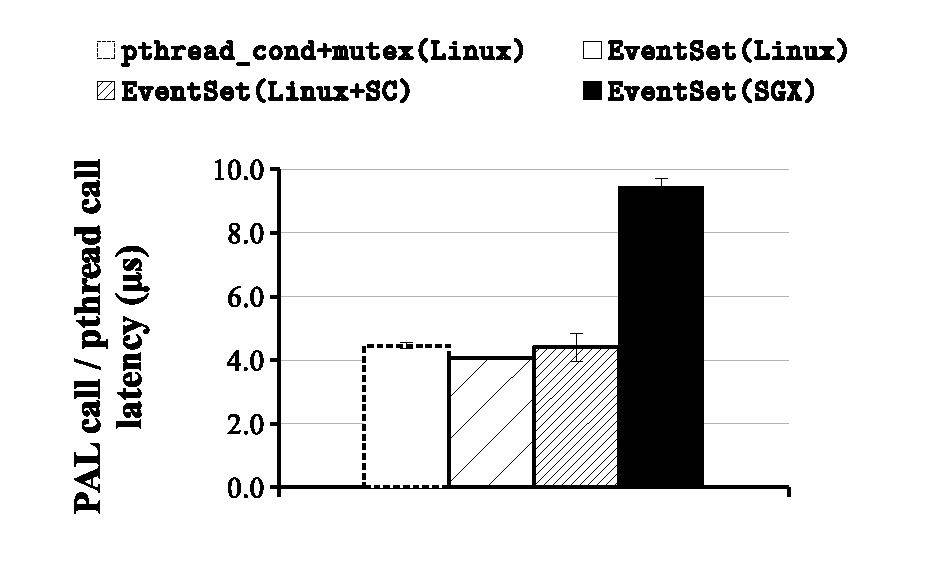
\includegraphics[height=10em]{event-latency}
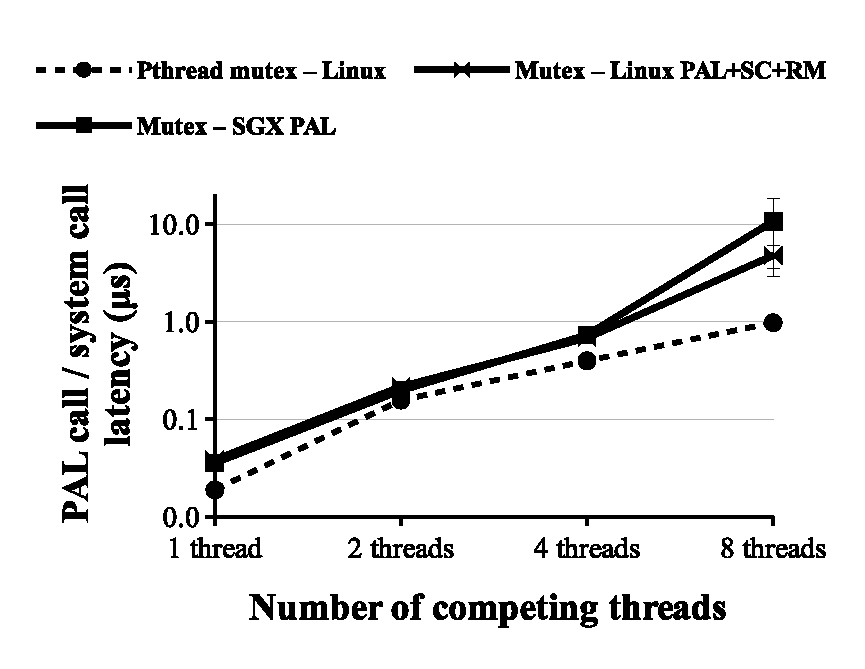
\includegraphics[height=10em]{mutex-latency}
}
\parbox{0.49\textwidth}{\centering\bf (a) signal an event}
\parbox{0.49\textwidth}{\centering\bf (b) competing a mutex among N threads}
\caption{Latency of (a) signaling an event and (b) competing a mutex among N threads (N: 1 to 8).
Lower is better.
The comparison is between (1) pthread condition variables and mutexes on Linux; (2) Notification events and mutexes on the Linux PAL, with and without a \seccomp{} filter ({\bf +SC}) and reference monitor ({\bf +RM}); (3) the same abstractions on the SGX PAL.}
\label{fig:eval:pal:sched-latency}
\end{figure*}




\paragraph{Events and mutexes.}
Figure~\ref{fig:eval:pal:sched-latency} (a)
shows the latency of signaling notification events
on the Linux and SGX PALs.
For a native Linux process, the pthread library
provide primitives similar to notification events in \thehostabi{},
using a combination
of conditional variables and mutexes.
In fact, the latency of event signaling on the Linux PAL
is slightly lower than updating a pthread conditional variable,
with extra a \roughly{}10\% overhead
if the \seccomp{} filter and reference monitor is enabled.
For the SGX PAL, the overhead on signaling an event
The overhead on the SGX PAL
is \roughly{}130\%,
and mostly contributes to the cost of exiting the enclave to call \syscall{futex}.




The latency of acquiring and releasing a mutex,
as shown in Figure~\ref{fig:eval:pal:sched-latency} (b),
is not scalable when multiple threads
access the same mutex.
Within a single thread,
acquiring and releasing a PAL mutex requires no \syscall{futex} calls
but simply updating a counter
in the mutex handle.
If the thread number is increased to two,
the latency of acquiring and releasing a PAL mutex may still be low
because
the Linux PAL always spin for a few rounds to check if
other thread has released the mutex.
Afterward, if the mutex is still locked,
the Linux PAL will block voluntarily,
by calling \syscall{futex} with \code{FUTEX\_WAIT}.
With eight threads trying to acquire the same mutex, the latency of acquring and releasing the mutex
is up to \roughly{}10\usec{}, or 286\% upon the latency of a pthread mutex.
 



